\documentclass{standalone}
\usepackage{pgfplots}
\pgfplotsset{compat=1.18}

\begin{document}

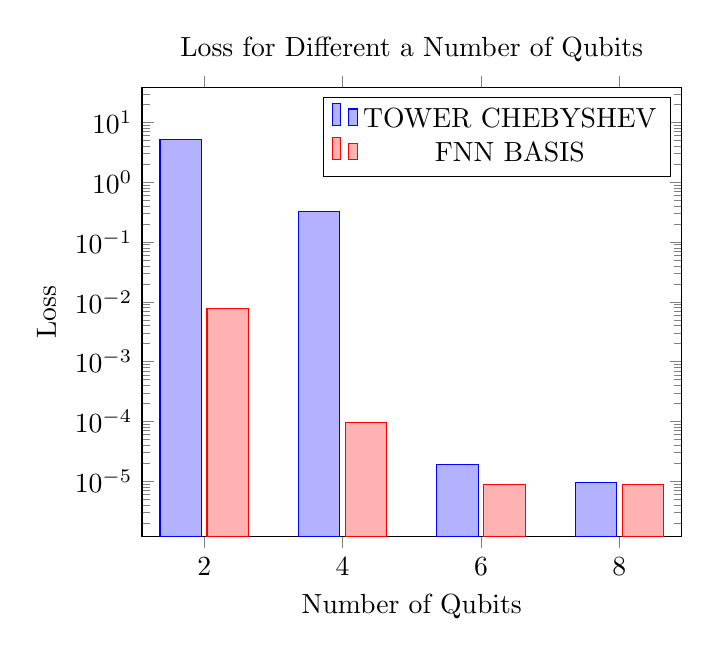
\begin{tikzpicture}
\begin{axis}[
    ybar,
    bar width=15pt,
    enlargelimits=0.15,
    ylabel={Loss},
    xlabel={Number of Qubits},
    symbolic x coords={2, 4, 6, 8},
    xtick=data,
    ymin=0,
    title={Loss for Different a Number of Qubits},
    log origin=infty,
    ymode=log,
]
\addplot coordinates {(2,5.1607) (4,0.3203) (6,1.8885e-05) (8,9.6682e-06)};
\addplot coordinates {(2,0.0077) (4,9.7179e-05) (6,8.8285e-06) (8,8.8918e-06)};

\legend{TOWER CHEBYSHEV, FNN BASIS}
\end{axis}
\end{tikzpicture}

\end{document}
